\section{Elsevier}
\subsection{ALEPH}
\pgfplotstabletypeset[
col sep=comma,
string type,
every head row/.style={%
	before row={\toprule\addlinespace
%		\multicolumn{10}{c}{ALEPH}\\
	},
	after row=\addlinespace\midrule\addlinespace
},
every last row/.style={after row=\addlinespace\bottomrule},
columns/FOLD/.style={column name=FOLD, column type=c},
columns/TP/.style={column name=TP, column type=c},
columns/TN/.style={column name=TN, column type=c},
columns/FP/.style={column name=FP, column type=c},
columns/FN/.style={column name=FN, column type=c},
columns/precision/.style={column name=precision, column type=c},
columns/recall/.style={column name=recall, column type=c},
columns/F-Measure/.style={column name=F-Measure, column type=c},
columns/Acc/.style={column name=Accuracy, column type=c},
columns/Err/.style={column name=Error, column type=c},
]{csv/elsevier/aleph.csv}


\subsection{PROGOL}
\pgfplotstabletypeset[
col sep=comma,
string type,
every head row/.style={%
	before row={\toprule\addlinespace
%		\multicolumn{10}{c}{PROGOL}\\
	},
	after row=\addlinespace\midrule\addlinespace
},
every last row/.style={after row=\addlinespace\bottomrule},
columns/FOLD/.style={column name=FOLD, column type=c},
columns/TP/.style={column name=TP, column type=c},
columns/TN/.style={column name=TN, column type=c},
columns/FP/.style={column name=FP, column type=c},
columns/FN/.style={column name=FN, column type=c},
columns/precision/.style={column name=precision, column type=c},
columns/recall/.style={column name=recall, column type=c},
columns/F-Measure/.style={column name=F-Measure, column type=c},
columns/Acc/.style={column name=Accuracy, column type=c},
columns/Err/.style={column name=Error, column type=c},
]{csv/elsevier/progol.csv}

\subsection{FOIL}
\pgfplotstabletypeset[
col sep=comma,
string type,
every head row/.style={%
	before row={\toprule\addlinespace
%		\multicolumn{10}{c}{FOIL}\\
	},
	after row=\addlinespace\midrule\addlinespace
},
every last row/.style={after row=\addlinespace\bottomrule},
columns/FOLD/.style={column name=FOLD, column type=c},
columns/TP/.style={column name=TP, column type=c},
columns/TN/.style={column name=TN, column type=c},
columns/FP/.style={column name=FP, column type=c},
columns/FN/.style={column name=FN, column type=c},
columns/precision/.style={column name=precision, column type=c},
columns/recall/.style={column name=recall, column type=c},
columns/F-Measure/.style={column name=F-Measure, column type=c},
columns/Acc/.style={column name=Accuracy, column type=c},
columns/Err/.style={column name=Error, column type=c},
]{csv/elsevier/foil.csv}

\subsection{Grafici}
\subsubsection{Precision}
\begin{figure}[hbtp]
	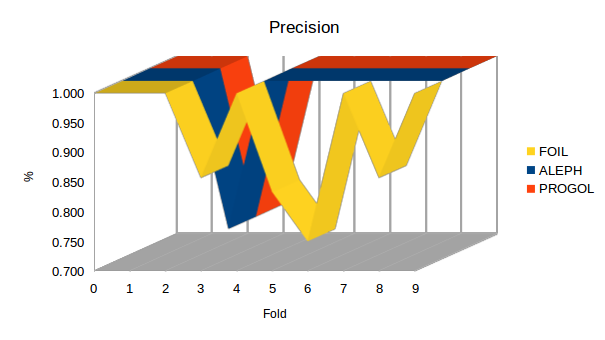
\includegraphics[width=1.2\textwidth]{img/datasetGraph/elsevier/precision.png}
	\label{Elsevier-Precision}
\end{figure}
\subsubsection{Recall}
\begin{figure}[hbtp]
	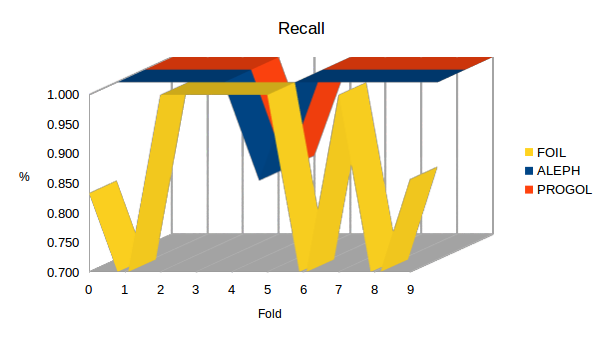
\includegraphics[width=1.2\textwidth]{img/datasetGraph/elsevier/recall.png}
	\label{Elsevier-Recall}
\end{figure}
\subsubsection{F-Measure}
\begin{figure}[hbtp]
	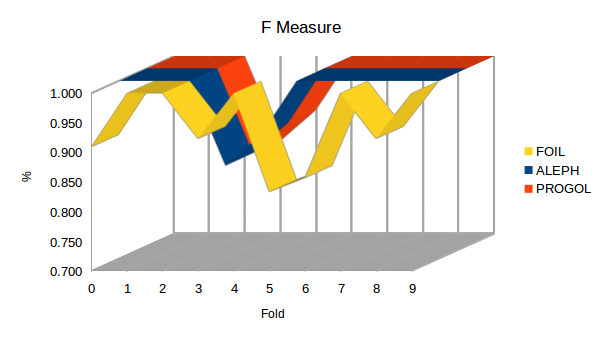
\includegraphics[width=1.2\textwidth]{img/datasetGraph/elsevier/fm.png}
	\label{Elsevier-F-measure}
\end{figure}
\subsubsection{Accuracy}
\begin{figure}[hbtp]
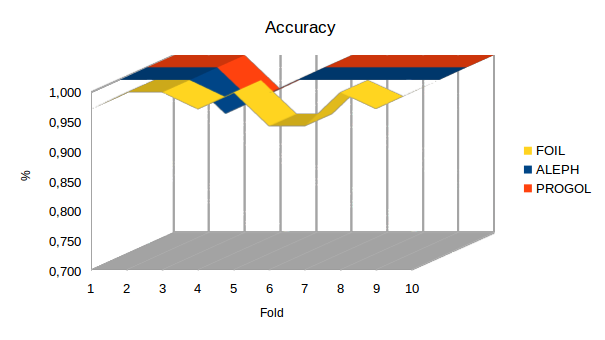
\includegraphics[width=1.2\textwidth]{img/datasetGraph/elsevier/accuracy.png}
\label{Elsevier-Accuracy}
\end{figure}
\subsubsection{Error}
\begin{figure}[hbtp]
	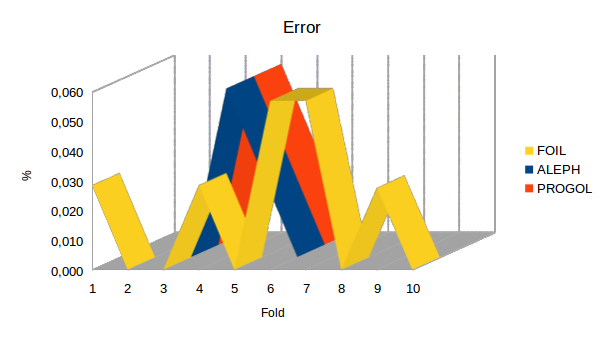
\includegraphics[width=1.2\textwidth]{img/datasetGraph/elsevier/error.png}
	\label{Elsevier-Error}
\end{figure}

\section{jmlr}
\subsection{ALEPH}
\pgfplotstabletypeset[
col sep=comma,
string type,
every head row/.style={%
	before row={\toprule\addlinespace
		%		\multicolumn{10}{c}{ALEPH}\\
	},
	after row=\addlinespace\midrule\addlinespace
},
every last row/.style={after row=\addlinespace\bottomrule},
columns/FOLD/.style={column name=FOLD, column type=c},
columns/TP/.style={column name=TP, column type=c},
columns/TN/.style={column name=TN, column type=c},
columns/FP/.style={column name=FP, column type=c},
columns/FN/.style={column name=FN, column type=c},
columns/precision/.style={column name=precision, column type=c},
columns/recall/.style={column name=recall, column type=c},
columns/F-Measure/.style={column name=F-Measure, column type=c},
columns/Acc/.style={column name=Accuracy, column type=c},
columns/Err/.style={column name=Error, column type=c},
]{csv/jmlr/aleph.csv}

\subsection{PROGOL}
\pgfplotstabletypeset[
col sep=comma,
string type,
every head row/.style={%
	before row={\toprule\addlinespace
		%		\multicolumn{10}{c}{PROGOL}\\
	},
	after row=\addlinespace\midrule\addlinespace
},
every last row/.style={after row=\addlinespace\bottomrule},
columns/FOLD/.style={column name=FOLD, column type=c},
columns/TP/.style={column name=TP, column type=c},
columns/TN/.style={column name=TN, column type=c},
columns/FP/.style={column name=FP, column type=c},
columns/FN/.style={column name=FN, column type=c},
columns/precision/.style={column name=precision, column type=c},
columns/recall/.style={column name=recall, column type=c},
columns/F-Measure/.style={column name=F-Measure, column type=c},
columns/Acc/.style={column name=Accuracy, column type=c},
columns/Err/.style={column name=Error, column type=c},
]{csv/jmlr/progol.csv}

\subsection{FOIL}
\pgfplotstabletypeset[
col sep=comma,
string type,
every head row/.style={%
	before row={\toprule\addlinespace
		%		\multicolumn{10}{c}{FOIL}\\
	},
	after row=\addlinespace\midrule\addlinespace
},
every last row/.style={after row=\addlinespace\bottomrule},
columns/FOLD/.style={column name=FOLD, column type=c},
columns/TP/.style={column name=TP, column type=c},
columns/TN/.style={column name=TN, column type=c},
columns/FP/.style={column name=FP, column type=c},
columns/FN/.style={column name=FN, column type=c},
columns/precision/.style={column name=precision, column type=c},
columns/recall/.style={column name=recall, column type=c},
columns/F-Measure/.style={column name=F-Measure, column type=c},
columns/Acc/.style={column name=Accuracy, column type=c},
columns/Err/.style={column name=Error, column type=c},
]{csv/jmlr/foil.csv}

\subsection{Grafici}
\subsubsection{Precision}
\begin{figure}[hbtp]
	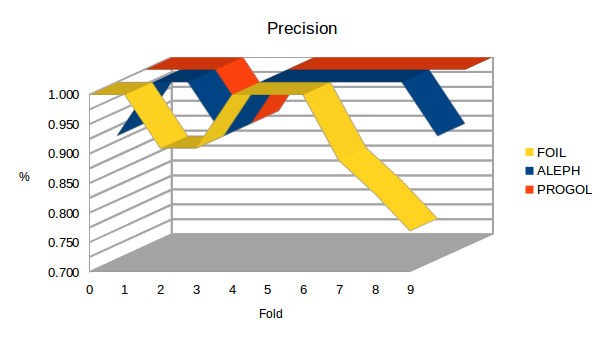
\includegraphics[width=1.2\textwidth]{img/datasetGraph/jmlr/precision.png}
	\label{JMLR-Precision}
\end{figure}
\subsubsection{Recall}
\begin{figure}[hbtp]
	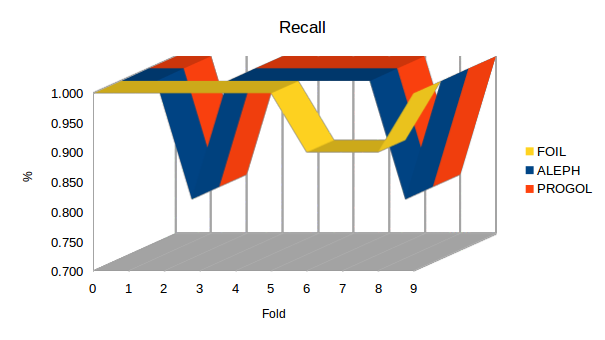
\includegraphics[width=1.2\textwidth]{img/datasetGraph/jmlr/recall.png}
	\label{JMLR-Recall}
\end{figure}
\subsubsection{F-Measure}
\begin{figure}[hbtp]
	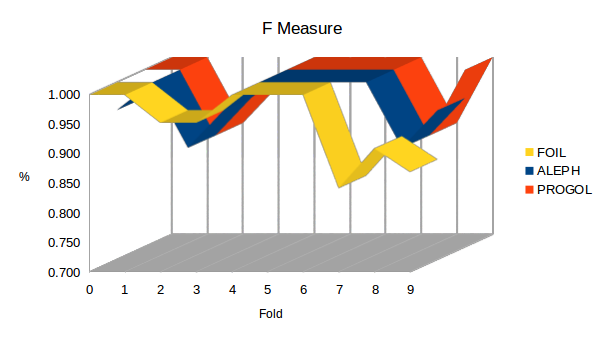
\includegraphics[width=1.2\textwidth]{img/datasetGraph/jmlr/fm.png}
	\label{JMLR-F-measure}
\end{figure}
\subsubsection{Accuracy}
\begin{figure}[hbtp]
	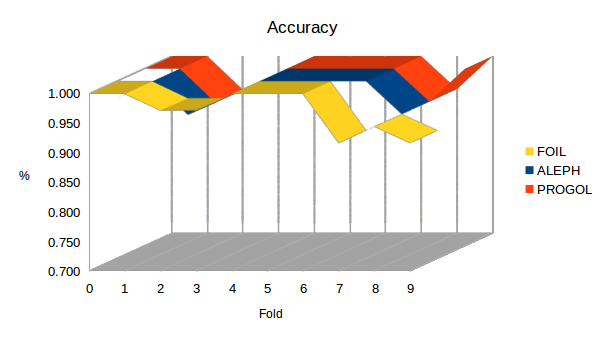
\includegraphics[width=1.2\textwidth]{img/datasetGraph/jmlr/accuracy.png}
	\label{JMLR-Accuracy}
\end{figure}
\subsubsection{Error}
\begin{figure}[hbtp]
	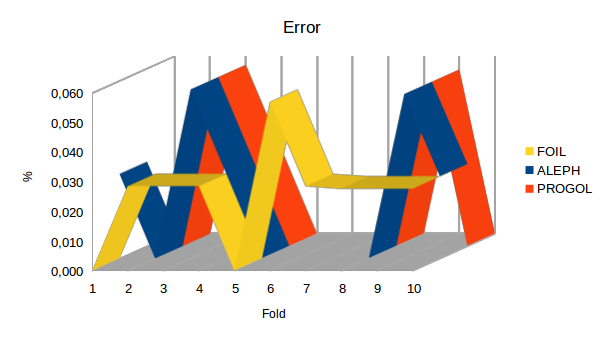
\includegraphics[width=1.2\textwidth]{img/datasetGraph/jmlr/error.png}
	\label{JMLR-Error}
\end{figure}

\section{svln}
\subsection{ALEPH}
\pgfplotstabletypeset[
col sep=comma,
string type,
every head row/.style={%
	before row={\toprule\addlinespace
		%		\multicolumn{10}{c}{ALEPH}\\
	},
	after row=\addlinespace\midrule\addlinespace
},
every last row/.style={after row=\addlinespace\bottomrule},
columns/FOLD/.style={column name=FOLD, column type=c},
columns/TP/.style={column name=TP, column type=c},
columns/TN/.style={column name=TN, column type=c},
columns/FP/.style={column name=FP, column type=c},
columns/FN/.style={column name=FN, column type=c},
columns/precision/.style={column name=precision, column type=c},
columns/recall/.style={column name=recall, column type=c},
columns/F-Measure/.style={column name=F-Measure, column type=c},
columns/Acc/.style={column name=Accuracy, column type=c},
columns/Err/.style={column name=Error, column type=c},
]{csv/svln/aleph.csv}

\subsection{PROGOL}
\pgfplotstabletypeset[
col sep=comma,
string type,
every head row/.style={%
	before row={\toprule\addlinespace
		%		\multicolumn{10}{c}{PROGOL}\\
	},
	after row=\addlinespace\midrule\addlinespace
},
every last row/.style={after row=\addlinespace\bottomrule},
columns/FOLD/.style={column name=FOLD, column type=c},
columns/TP/.style={column name=TP, column type=c},
columns/TN/.style={column name=TN, column type=c},
columns/FP/.style={column name=FP, column type=c},
columns/FN/.style={column name=FN, column type=c},
columns/precision/.style={column name=precision, column type=c},
columns/recall/.style={column name=recall, column type=c},
columns/F-Measure/.style={column name=F-Measure, column type=c},
columns/Acc/.style={column name=Accuracy, column type=c},
columns/Err/.style={column name=Error, column type=c},
]{csv/svln/progol.csv}

\subsection{FOIL}
\pgfplotstabletypeset[
col sep=comma,
string type,
every head row/.style={%
	before row={\toprule\addlinespace
		%		\multicolumn{10}{c}{FOIL}\\
	},
	after row=\addlinespace\midrule\addlinespace
},
every last row/.style={after row=\addlinespace\bottomrule},
columns/FOLD/.style={column name=FOLD, column type=c},
columns/TP/.style={column name=TP, column type=c},
columns/TN/.style={column name=TN, column type=c},
columns/FP/.style={column name=FP, column type=c},
columns/FN/.style={column name=FN, column type=c},
columns/precision/.style={column name=precision, column type=c},
columns/recall/.style={column name=recall, column type=c},
columns/F-Measure/.style={column name=F-Measure, column type=c},
columns/Acc/.style={column name=Accuracy, column type=c},
columns/Err/.style={column name=Error, column type=c},
]{csv/svln/foil.csv}

\subsection{Grafici}
\subsubsection{Precision}
\begin{figure}[hbtp]
	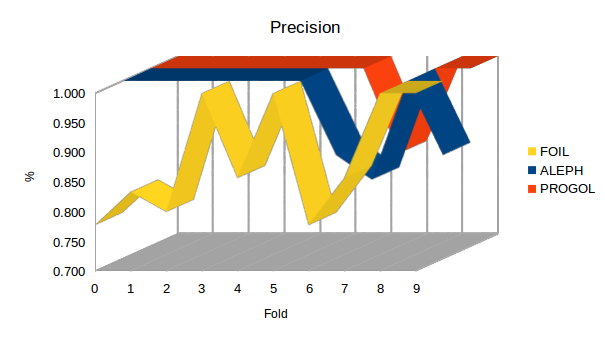
\includegraphics[width=1.2\textwidth]{img/datasetGraph/svln/precision.png}
	\label{svln-Precision}
\end{figure}
\subsubsection{Recall}
\begin{figure}[hbtp]
	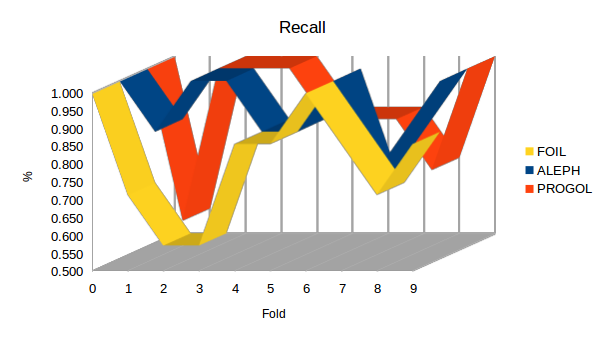
\includegraphics[width=1.2\textwidth]{img/datasetGraph/svln/recall.png}
	\label{svln-Recall}
\end{figure}
\subsubsection{F-Measure}
\begin{figure}[hbtp]
	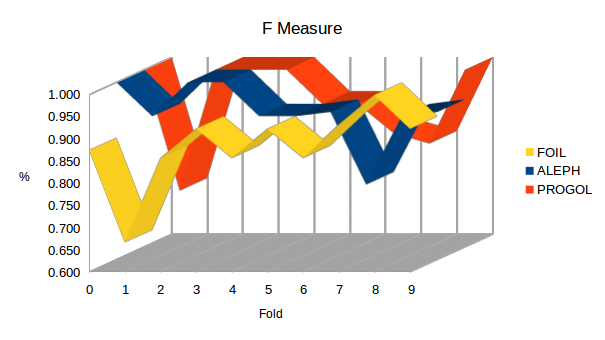
\includegraphics[width=1.2\textwidth]{img/datasetGraph/svln/fm.png}
	\label{svln-F-measure}
\end{figure}
\subsubsection{Accuracy}
\begin{figure}[hbtp]
	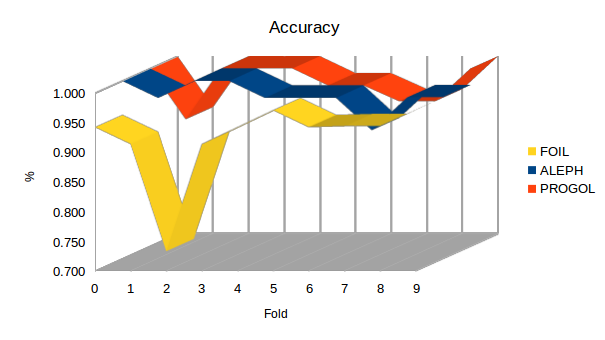
\includegraphics[width=1.2\textwidth]{img/datasetGraph/svln/accuracy.png}
	\label{svln-Accuracy}
\end{figure}
\subsubsection{Error}
\begin{figure}[hbtp]
	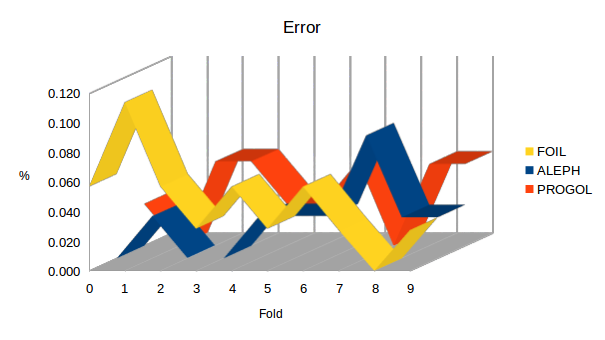
\includegraphics[width=1.2\textwidth]{img/datasetGraph/svln/error.png}
	\label{svln-Error}
\end{figure}

\section{MLJ - discretizzato}
\subsection{ALEPH}
\pgfplotstabletypeset[
col sep=comma,
string type,
every head row/.style={%
	before row={\toprule\addlinespace
		%		\multicolumn{10}{c}{ALEPH}\\
	},
	after row=\addlinespace\midrule\addlinespace
},
every last row/.style={after row=\addlinespace\bottomrule},
columns/FOLD/.style={column name=FOLD, column type=c},
columns/TP/.style={column name=TP, column type=c},
columns/TN/.style={column name=TN, column type=c},
columns/FP/.style={column name=FP, column type=c},
columns/FN/.style={column name=FN, column type=c},
columns/precision/.style={column name=precision, column type=c},
columns/recall/.style={column name=recall, column type=c},
columns/F-Measure/.style={column name=F-Measure, column type=c},
columns/Acc/.style={column name=Accuracy, column type=c},
columns/Err/.style={column name=Error, column type=c},
]{csv/mlj/discr/aleph.csv}

\subsection{PROGOL}
\pgfplotstabletypeset[
col sep=comma,
string type,
every head row/.style={%
	before row={\toprule\addlinespace
		%		\multicolumn{10}{c}{PROGOL}\\
	},
	after row=\addlinespace\midrule\addlinespace
},
every last row/.style={after row=\addlinespace\bottomrule},
columns/FOLD/.style={column name=FOLD, column type=c},
columns/TP/.style={column name=TP, column type=c},
columns/TN/.style={column name=TN, column type=c},
columns/FP/.style={column name=FP, column type=c},
columns/FN/.style={column name=FN, column type=c},
columns/precision/.style={column name=precision, column type=c},
columns/recall/.style={column name=recall, column type=c},
columns/F-Measure/.style={column name=F-Measure, column type=c},
columns/Acc/.style={column name=Accuracy, column type=c},
columns/Err/.style={column name=Error, column type=c},
]{csv/mlj/discr/progol.csv}

\subsection{FOIL}
\pgfplotstabletypeset[
col sep=comma,
string type,
every head row/.style={%
	before row={\toprule\addlinespace
		%		\multicolumn{10}{c}{FOIL}\\
	},
	after row=\addlinespace\midrule\addlinespace
},
every last row/.style={after row=\addlinespace\bottomrule},
columns/FOLD/.style={column name=FOLD, column type=c},
columns/TP/.style={column name=TP, column type=c},
columns/TN/.style={column name=TN, column type=c},
columns/FP/.style={column name=FP, column type=c},
columns/FN/.style={column name=FN, column type=c},
columns/precision/.style={column name=precision, column type=c},
columns/recall/.style={column name=recall, column type=c},
columns/F-Measure/.style={column name=F-Measure, column type=c},
columns/Acc/.style={column name=Accuracy, column type=c},
columns/Err/.style={column name=Error, column type=c},
]{csv/mlj/discr/foil.csv}


\subsection{Grafici}
\subsubsection{Precision}
\begin{figure}[hbtp]
	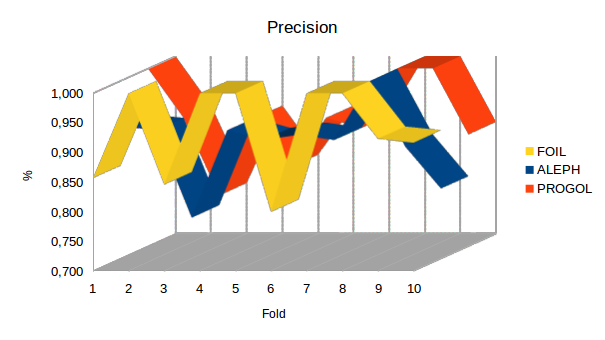
\includegraphics[width=1.2\textwidth]{img/datasetGraph/mlj/discr/precision.png}
	\label{mljdiscr-Precision}
\end{figure}
\subsubsection{Recall}
\begin{figure}[hbtp]
	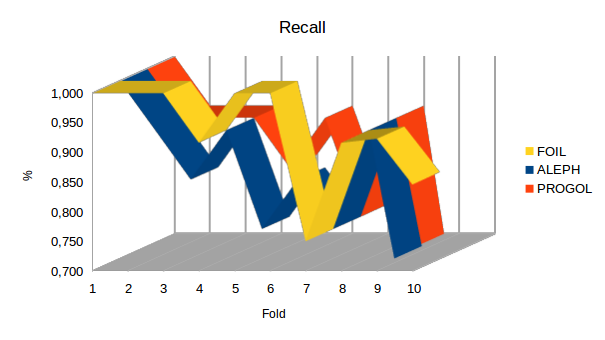
\includegraphics[width=1.2\textwidth]{img/datasetGraph/mlj/discr/recall.png}
	\label{mljdiscr-Recall}
\end{figure}
\subsubsection{F-Measure}
\begin{figure}[hbtp]
	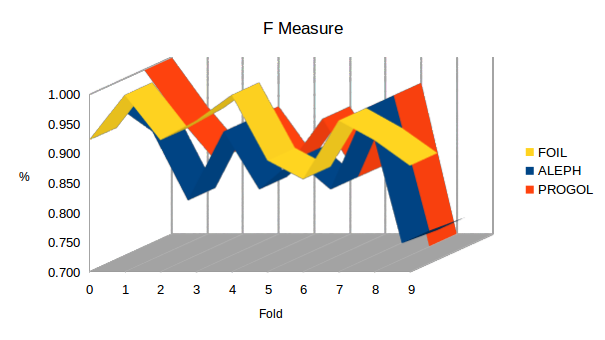
\includegraphics[width=1.2\textwidth]{img/datasetGraph/mlj/discr/fm.png}
	\label{mljdiscr-F-measure}
\end{figure}
\subsubsection{Accuracy}
\begin{figure}[hbtp]
	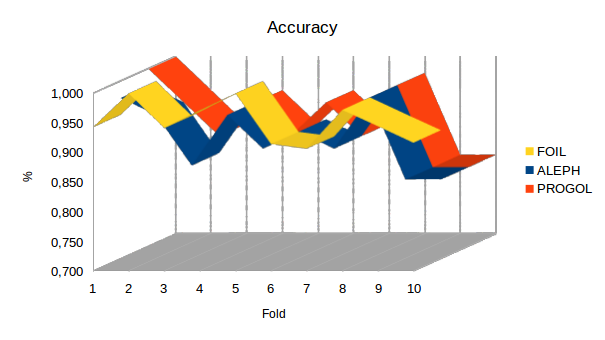
\includegraphics[width=1.2\textwidth]{img/datasetGraph/mlj/discr/accuracy.png}
	\label{mljdiscr-Accuracy}
\end{figure}
\subsubsection{Error}
\begin{figure}[hbtp]
	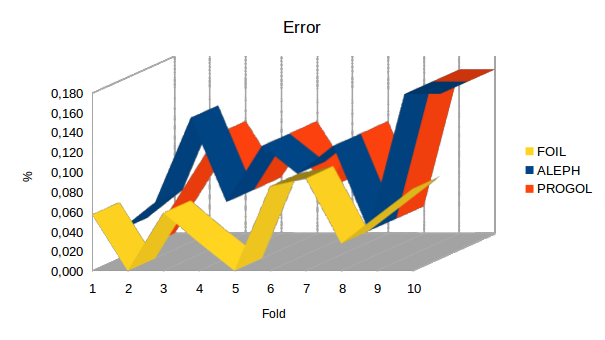
\includegraphics[width=1.2\textwidth]{img/datasetGraph/mlj/discr/error.png}
	\label{mljdiscr-Error}
\end{figure}

\section{MLJ - non discretizzato}
\subsection{ALEPH}
\pgfplotstabletypeset[
col sep=comma,
string type,
every head row/.style={%
	before row={\toprule\addlinespace
		%		\multicolumn{10}{c}{ALEPH}\\
	},
	after row=\addlinespace\midrule\addlinespace
},
every last row/.style={after row=\addlinespace\bottomrule},
columns/FOLD/.style={column name=FOLD, column type=c},
columns/TP/.style={column name=TP, column type=c},
columns/TN/.style={column name=TN, column type=c},
columns/FP/.style={column name=FP, column type=c},
columns/FN/.style={column name=FN, column type=c},
columns/precision/.style={column name=precision, column type=c},
columns/recall/.style={column name=recall, column type=c},
columns/F-Measure/.style={column name=F-Measure, column type=c},
columns/Acc/.style={column name=Accuracy, column type=c},
columns/Err/.style={column name=Error, column type=c},
]{csv/mlj/nodiscr/aleph.csv}

\subsection{PROGOL}
\pgfplotstabletypeset[
col sep=comma,
string type,
every head row/.style={%
	before row={\toprule\addlinespace
		%		\multicolumn{10}{c}{PROGOL}\\
	},
	after row=\addlinespace\midrule\addlinespace
},
every last row/.style={after row=\addlinespace\bottomrule},
columns/FOLD/.style={column name=FOLD, column type=c},
columns/TP/.style={column name=TP, column type=c},
columns/TN/.style={column name=TN, column type=c},
columns/FP/.style={column name=FP, column type=c},
columns/FN/.style={column name=FN, column type=c},
columns/precision/.style={column name=precision, column type=c},
columns/recall/.style={column name=recall, column type=c},
columns/F-Measure/.style={column name=F-Measure, column type=c},
columns/Acc/.style={column name=Accuracy, column type=c},
columns/Err/.style={column name=Error, column type=c},
]{csv/mlj/nodiscr/progol.csv}

\subsection{FOIL}

\pgfplotstabletypeset[
col sep=comma,
string type,
every head row/.style={%
	before row={\toprule\addlinespace
		%		\multicolumn{10}{c}{FOIL}\\
	},
	after row=\addlinespace\midrule\addlinespace
},
every last row/.style={after row=\addlinespace\bottomrule},
columns/FOLD/.style={column name=FOLD, column type=c},
columns/TP/.style={column name=TP, column type=c},
columns/TN/.style={column name=TN, column type=c},
columns/FP/.style={column name=FP, column type=c},
columns/FN/.style={column name=FN, column type=c},
columns/precision/.style={column name=precision, column type=c},
columns/recall/.style={column name=recall, column type=c},
columns/F-Measure/.style={column name=F-Measure, column type=c},
columns/Acc/.style={column name=Accuracy, column type=c},
columns/Err/.style={column name=Error, column type=c}
]{csv/mlj/nodiscr/foil.csv}

\subsection{Grafici}
\subsubsection{Precision}
\begin{figure}[hbtp]
	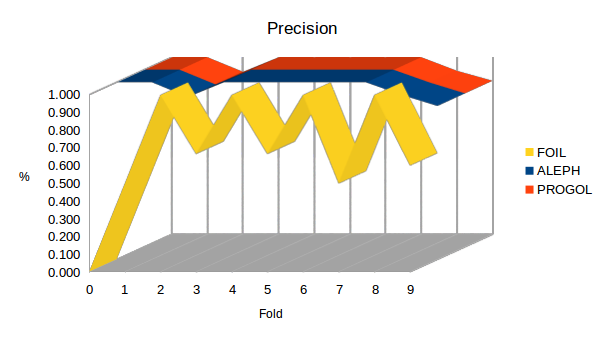
\includegraphics[width=1.2\textwidth]{img/datasetGraph/mlj/nodiscr/precision.png}
	\label{mljnodiscr-Precision}
\end{figure}
\subsubsection{Recall}
\begin{figure}[hbtp]
	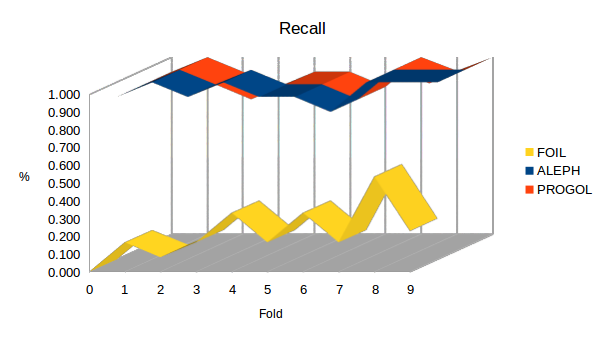
\includegraphics[width=1.2\textwidth]{img/datasetGraph/mlj/nodiscr/recall.png}
	\label{mljnodiscr-Recall}
\end{figure}
\subsubsection{F-Measure}
\begin{figure}[hbtp]
	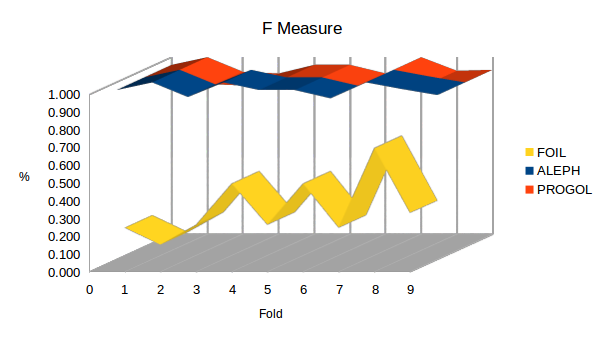
\includegraphics[width=1.2\textwidth]{img/datasetGraph/mlj/nodiscr/fm.png}
	\label{mljnodiscr-F-measure}
\end{figure}
\subsubsection{Accuracy}
\begin{figure}[hbtp]
	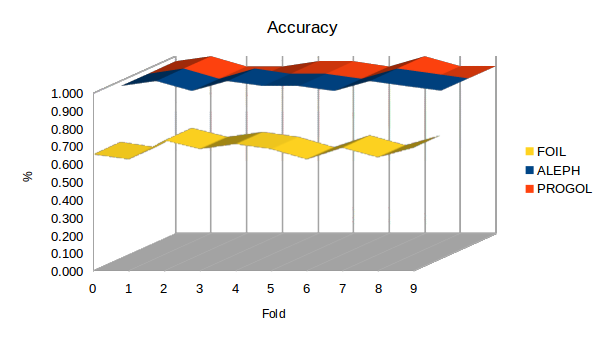
\includegraphics[width=1.2\textwidth]{img/datasetGraph/mlj/nodiscr/accuracy.png}
	\label{mljnodiscr-Accuracy}
\end{figure}
\subsubsection{Error}
\begin{figure}[hbtp]
	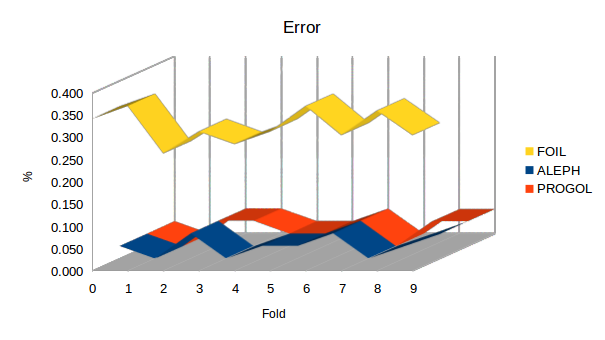
\includegraphics[width=1.2\textwidth]{img/datasetGraph/mlj/nodiscr/error.png}
	\label{mljnodiscr-Error}
\end{figure}